\subsection{Write Back Stage}

\begin{figure}[H]
    \centering
    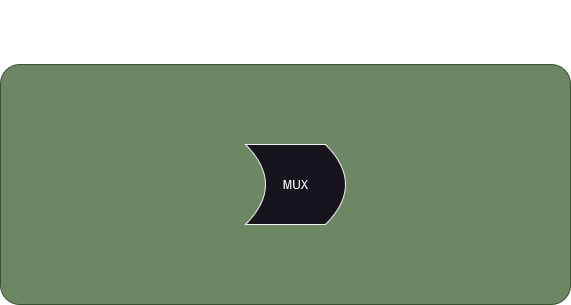
\includegraphics[width=0.75\textwidth]{../diagrams/writeback/wb_stage.png}
    \caption{Write Back stage}
    \label{fig:wb_stage}
\end{figure}

The writeback stage is the fifth and last stage of the pipeline. It is the simpler stage that contains only one module,
a simple 3 entry mux that choose which data between the Branch Unit, the ALU and the LSU will be written back to the 
register file.
